\documentclass[twoside,11pt]{homework}
\usepackage{listings}
\usepackage{xcolor}
\usepackage{graphicx} 

\coursename{COMS 4771 Machine Learning (2018 Fall)} 

\studname{Jing Qian}    % YOUR NAME GOES HERE
\studmail{jq2282@columbia.edu}% YOUR UNI GOES HERE
\hwNo{0}                   % THE HOMEWORK NUMBER GOES HERE
\date{\today} % DATE GOES HERE


\begin{document}
\maketitle

\section*{Problem 1.1}
(i) %The marginal distribution of $X$ is: 
%
\begin{equation}
\begin{split}
\mathrm{Pr}[X=1] = \sum_y \mathrm{Pr}[X=1, Y=y] = 0.2 + 0.2 + 0.3 = 0.7 \\
\mathrm{Pr}[X=2] = \sum_y \mathrm{Pr}[X=2, Y=y] = 0.1 + 0.1 + 0.1 = 0.3
\end{split}
%\label{E1}
\end{equation}
%

\noindent (ii) 
%
\begin{equation}
\mathrm{Pr}[Y=1|X=2] = \frac{\mathrm{Pr}[Y=1, X=2] }{\mathrm{Pr}[X=2] } = \frac{1}{3}
\end{equation}
%

\noindent (iii) 
 %
\begin{equation}
\begin{split}
\mathrm{Pr}[X=1|Y=3] = \frac{0.3}{0.3+0.1} = 0.75\\
\mathrm{Pr}[X=2|Y=3] = \frac{0.1}{0.3+0.1} = 0.25
\end{split}
%\label{E1}
\end{equation}
%
 %
\begin{equation}
\bbE[f(X)|Y=3] = 1^2 * \mathrm{Pr}[X=1|Y=3] + 2^2 * \mathrm{Pr}[X=2|Y=3] = 1.75
%\label{E1}
\end{equation}
%

%%%%%%%%%%%%%%%%%%%%%%%%%%%%%%%%%%%%%%
\section*{Problem 1.2}
(i) To be a probability distribution, $g_\theta$ has to satisfy following two conditions:
1) $g_\theta(x) \geq 0$ for any $x \in [0, \infty)$;
2) $\int_0^{\infty} g_{\theta} (x) dx = 1$.

Since $\theta > 0$ and $e^{-\frac{x}{\theta}} > 0$, $g_\theta > 0$. 
First condition is satisfied.
 %
\begin{equation}
%\begin{split}
\int_0^{\infty} g_{\theta} (x) dx = \int_0^{\infty}\frac{1}{\theta}\ e^{-\frac{x}{\theta}} dx
= \int_0^{\infty} e^{-y} dy
= 1 
%\end{split}
\end{equation}
%
where $y = \frac{x}{\theta}$. Second condition is satisfied too. So $g_\theta$ is a probability distribution.

\noindent (ii)
%
\begin{equation}
%\begin{split}
\bbE􏰁[g_{\theta}] = \int_0^{\infty} x\ g_{\theta} (x)\ dx 
=  \int_0^{\infty} \frac{x}{\theta}\ e^{-\frac{x}{\theta}} dx
= \theta \int_0^{\infty}y\ e^{-y} dy 
= \theta 
%\end{split}
\end{equation}
%
where $y = \frac{x}{\theta}$.
\vspace{3 mm}

\noindent (iii)
%
\begin{equation}
\begin{split}
\rm􏰁{var}(g_{\theta})&= \int_0^{\infty} (x - \bbE􏰁[g_{\theta}])^2 g_{\theta} (x)\ dx \\
&= \int_0^{\infty} \frac{(x - \theta)^2 }{\theta}\ e^{-\frac{x}{\theta}} dx \\
&= \theta^2 \int_0^{\infty}y^2\ e^{-y} dy - 2\theta^2 \int_0^{\infty}y\ e^{-y} dy + \theta^2\int_0^{\infty}\ e^{-y} dy \\
%&=  2\theta^2 \int_0^{\infty}y\ e^{-y} dy - 2\theta^2 \int_0^{\infty}y\ e^{-y} dy + \theta^2\int_0^{\infty}\ e^{-y} dy  \\
&= \theta^2
\end{split}
\end{equation}
%

%%%%%%%%%%%%%%%%%%%%%%%%%%%%%%%%%%%%%%
\section*{Problem 1.3}
Considering that $X$ and $Y$ are jointly distributed Gaussian random variables, $X+Y$ is still Gaussian distributed. 
%
\begin{equation}
\begin{split}
\bbE􏰁[X+Y] &= \sum_x \sum_y (x+y) \rm{Pr} (X=x, Y=y)  \\
&= \sum_x \sum_y x \rm{Pr} (X=x, Y=y) + \sum_x \sum_y y \rm{Pr} (X=x, Y=y) \\
&= \sum_x x \rm{Pr} (X=x) + \sum_y y \rm{Pr} (Y=y) \\
&= \bbE􏰁[X] + \bbE􏰁[Y] \\
&= 0
\end{split}
\end{equation}
%
%
\begin{equation}
\begin{split}
\rm􏰁{var}(X+Y)&= \bbE􏰁[(X+Y)^2] - \bbE􏰁[X+Y]^2 \\
&= \bbE[X^2] +\bbE[Y^2] + 2\bbE[XY] - (\bbE[X] + \bbE[Y])^2 \\
&= (\bbE[X^2] - \bbE[x]^2) + (\bbE[Y^2] - \bbE[Y]^2) + 2(\bbE[XY] - \bbE[X] \bbE[Y]) \\
&= \rm􏰁{var}(X) + \rm􏰁{var}(Y) + 2\rm􏰁{cov}(X, Y) \\
&= 6
\end{split}
\end{equation}
%
So $X+Y$ has Gaussian distribution with the mean 0 and variance 6, in other words, $N(0, 6)$.

%%%%%%%%%%%%%%%%%%%%%%%%%%%%%%%%%%%%%%
\section*{Problem 1.4}
For a fair coin, which means the possiblity of tossing a head is $\frac{1}{2}$ every time, 
the expected absolute difference between the number of heads H and that of tails T is:
%
\begin{equation}
%\begin{split}
\bbE􏰁[|H - T|] = \sum_{i=0}^{n} {n \choose i} (\frac{1}{2})^i (\frac{1}{2})^{n-i}\ |i - (n-i)|= \frac{1}{2^n} \sum_{i=0}^{n} {n \choose i}\ |2 i - n|
%\end{split}
\label{E1}
\end{equation}
%
where $i$ is the number of heads. Since ${n \choose i}\ |2 i - n| = {n \choose j}\ |2 j - n|$ while $j = n - i$, we have:
%
\begin{equation}
\sum_{i=0}^{n} {n \choose i}\ |2 i - n|= \left\{
\begin{aligned}
&2 \sum_{i=0}^{\frac{n}{2} - 1}  {n \choose i}\ (n - 2 i) + {n \choose n/2} (n - n) = 2 \sum_{i=0}^{\frac{n}{2} - 1}  {n \choose i}\ (n - 2 i),      & n\ \mathrm{ is\ even.} \\
&2 \sum_{i=0}^{\frac{n-1}{2}}  {n \choose i}\ (n - 2 i),     & n\ \mathrm{is\ odd.}
\end{aligned}
%\right
\label{E2}
\end{equation}
%

Since the odd case and even case have slight differences, we treat them seperately.
%
\begin{equation}
\begin{split}
\bbE_{\mathrm{even}}􏰁[|H - T|] &= \frac{1}{2^{(n-1)}} \sum_{i=0}^{\frac{n}{2} - 1}  {n \choose i} \ (n - 2 i) = \frac{1}{2^{(n-1)}} \sum_{i=0}^{\frac{n}{2} - 1} \frac{n!}{i!\ (n-i)!}\ [(n - i) - i]\\
&= \frac{1}{2^{(n-1)}}[\sum_{i=0}^{\frac{n}{2} - 1} \frac{n!}{i!\ (n-i)!}\ (n-i) - \sum_{i=0}^{\frac{n}{2} - 1} \frac{n!}{i!\ (n-i)!}\  i] \\
%&= \frac{1}{2^{(n-1)}}[\sum_{i=0}^{\frac{n}{2} - 1} \frac{n!}{i!\ (n-i-1)!} - \sum_{i=1}^{\frac{n}{2} - 1} \frac{n!}{(i-1)!\ (n-i)!}] \\
&= \frac{1}{2^{(n-1)}}[\sum_{i=0}^{\frac{n}{2} - 1} \frac{n!}{i!\ (n-i-1)!} - \sum_{j=0}^{\frac{n}{2} - 2} \frac{n!}{j!\ (n-j-1)!}]   
\end{split}
\label{E3}
\end{equation}
%
where $j = i - 1$.
After subtraction of the two summations in Eq.~\eqref{E3}, only the term $i = \frac{n}{2} -1$ remains.
%
\begin{equation}
\bbE_{\mathrm{even}}􏰁[|H - T|] = \frac{1}{2^{(n-1)}} \frac{n!}{(\frac{n}{2} -1)! (\frac{n}{2})!}= \frac{n}{2^n}\ \frac{n!}{((\frac{n}{2})!)^2}
\label{E4}
\end{equation}
%
Similarly, we could get the result when $n$ is an odd number:
%
\begin{equation}
\bbE􏰁[|H - T|] = \left\{
\begin{aligned}
& \frac{n}{2^n}\ \frac{n!}{((\frac{n}{2})!)^2},    & n\ \mathrm{ is\ even.} \\
& \frac{1}{2^{(n-1)}} \  \frac{n!}{((\frac{n-1}{2})!)^2},    & n\ \mathrm{is\ odd.}
\end{aligned}
\right
\label{E5}
\end{equation}
%

When $n \to \infty$, we could get an approximate value for Eq.~\eqref{E5} using Stirling's approximation for factorials.
%
\begin{equation}
\begin{split}
\bbE_{\mathrm{even}}􏰁[|H - T|] = \frac{n}{2^n}\ \frac{n!}{((\frac{n}{2})!)^2} \approx \frac{n}{2^n}\ \frac{\sqrt{2 \pi n}\ (\frac{n}{e})^n}{ \pi n (\frac{n}{2e})^n} = \sqrt{\frac{2n}{\pi}}
\end{split}
\label{E6}
\end{equation}
%
And
%
\begin{equation}
\begin{split}
\bbE_{\mathrm{odd}}􏰁[|H - T|] &=  \frac{1}{2^{(n-1)}} \  \frac{n!}{((\frac{n-1}{2})!)^2} \approx \frac{1}{2^{(n - 1)}}\ \frac{\sqrt{2 \pi n}\ (\frac{n}{e})^n}{\pi (n-1) (\frac{n-1}{2e})^{(n-1)}} \\
&= \sqrt{\frac{2n}{\pi}} \ \frac{1}{e}\ \frac{1}{(1-\frac{1}{n})^n} \\
&\approx \sqrt{\frac{2n}{\pi}} 
\end{split}
\end{equation}
%

So when independently toss a fair coin $n$ times, the expected absolute difference between the number of heads H and the number of tails T is about $\sqrt{\frac{2n}{\pi}} $.

\newpage
%%%%%%%%%%%%%%%%%%%%%%%%%%%%%%%%%%%%%%
\section*{Problem 2.1}
(i) Let A be a matrix contains vectors in the question and be transformed into row echelon form: 
%
\begin{equation}
\bf{A} = \left[ \begin{matrix} 1\ 2\ 3 \\ 2\ 8\ 10 \\ 3\ 3\ 6 \\ 4\ 2\ 6 \end{matrix} \right] 
\Longleftrightarrow \mathbf{V} = \left[ \begin{matrix} 1\ 0\ 0 \\ 0\ 1\ 0 \\ 0\ 0\ 0 \\ 0\ 0\ 0 \end{matrix} \right] 
\end{equation}
%
Since rank($\bf{A}$) = rank($\bf{V}$) =2, the dimension of the subspace $S$ is 2.
\vspace{3 mm}

\noindent(ii) To get the orthogonal linear projection of the point $\left(\begin{smallmatrix} 6\\5\\9\\2 \end{smallmatrix} \right)$ onto the subspace $S$, we need to calculate the orthonormal basis of subspace $S$ first.
From (i), we could get the orthonormal basis $( \mathbf{v_1, v_2}) $ of subspace $S$:
%
\begin{equation}
 ( \mathbf{v_1, v_2}) = \left(\left[\begin{matrix} 1\\0 \\0 \\0 \end{matrix}\right],  \left[\begin{matrix} 0\\1 \\ 0 \\ 0\end{matrix}\right] \right)
\end{equation}
%
Gram-Schmidt orthogonalization also works but the given orthonormal basis are much more complex.


%As the vector $\left(\begin{smallmatrix} 3\\10\\6\\6 \end{smallmatrix} \right)$ equals to the sum of the other two vectors, we could compute the orthonormal basis of $S$ only using these two vectors through Gram-Schmidt orthogonalization:
%%
%\begin{equation}
%\mathbf{V} = [ \mathbf{v_1, v_2}] = \left[\frac{1}{\sqrt{30}} \left[\begin{matrix} 1\\2 \\3 \\4 \end{matrix}\right],  \sqrt{\frac{6}{241}}\left[\begin{matrix} \frac{5}{6}\\\frac{17}{3} \\ -\frac{1}{2} \\ -\frac{8}{3}\end{matrix}\right] \right]
%\end{equation}
%%
So the projection P of given point $\mathbf{u} = \left(\begin{smallmatrix} 6\\5\\9\\2 \end{smallmatrix}\right)$ onto $S$ is:
%
\begin{equation}
\mathbf{P} = \sum_i \frac{<\bf{u}, \bf{v_i}>}{\bf{<v_i, v_i>}} \bf{v_i} = <\bf{u}, \bf{v_1}> \bf{v_1} +  <\bf{u}, \bf{v_2}> \bf{v_2} = \left(\begin{matrix} 6\\5\\0\\0 \end{matrix}\right).
\end{equation}
%
%In python, we could call scipy.linalg.orth to get the orthonormal basis of given matrix, which based on SVD, not Gram-Schmidt.


%%%%%%%%%%%%%%%%%%%%%%%%%%%%%%%%%%%%%%
\section*{Problem 2.2}
A square matrix is invertible if and only if none of its eigenvalues is zero. 
So to prove $\bf{A^{T}A + \rho I}$ is invertible, we could try to prove that all its eigenvalues are non-zero. Let $\lambda$ be one eigenvalue of matrix $\bf{A^{T}A + \rho I}$. 
Then we have:
%
\begin{equation}
\bf{det(A^{T}A + \rho I - \lambda I)} = 0 
\end{equation}
%
%\bf{det(A^{T}A) + det(\rho I) - det(\lambda I)} = 0 
So, 
%
\begin{equation}
\lambda = \bf{det(A^{T}A) }+ \rho 
\end{equation}
%
Let $\tilde{\lambda}$ and x be one eigenvalue and corresponding eigenvector of matrix $\bf{A^{T}A$. 
In other words, $\bf{A^{T}A x = \tilde{\lambda} x}$.
Then,
%
\begin{equation}
||\bf{Ax|| = (Ax)^T Ax = x^T A^T Ax = \tilde{\lambda} x^T x = \tilde{\lambda}}
\end{equation}
%
Since $ \bf{det(A^{T}A)} = \bf{\tilde{\lambda} = ||Ax|| \ge 0}$ and $\rho > 0$,
$\lambda = \bf{det(A^{T}A) }+ \rho > 0$.

Therefore, the matrix $\bf{A^{T}A + \rho I}$ is invertible because its eigenvalues are all positive. 

\newpage

%%%%%%%%%%%%%%%%%%%%%%%%%%%%%%%%%%%%%%
\section*{Problem 3.1}
(i) The function could be expanded as following:
%
\begin{equation}
\begin{split}
f (\bf{x}) &= \bf{||Ax - b||^2 + ||x||^2 = (Ax - b)^T (Ax - b) + x^T x} \\
&=\bf{ x^T A^T A x + x^T x - x^T A^T b - b^T A x + b^T b}
\end{split}
\end{equation}
%
Using the derivatives of matrices:
%
\begin{equation}
\begin{split}
\bf{\frac{\partial x^T B}{\partial x}} &=  \bf{\frac{\partial B^T x}{\partial x}} = B\\
\bf{\frac{\partial x^T B x}{\partial x}} &=  \bf{(B + B^T) x}\\
\bf{\frac{\partial x^T B x}{\partial x}} &=  \bf{2 x}
\end{split}
\end{equation}
%
We could get: 
%
\begin{equation}
\begin{split}
\nabla f (\bf{x}) &=  \frac{\partial (\bf{ x^T A^T A x + x^T x - x^T A^T b - b^T A x + b^T b})}{\partial \bf{x}} \\
&= \bf{2A^TA x + 2x - 2 A^Tb}
\end{split}
\end{equation}
%

%* Second method to do matrix derivation:
%%
%\begin{equation}
%\begin{split}
%f (\bf{x}) &= \bf{||Ax - b||^2 + ||x||^2 = (Ax - b)^T (Ax - b) + x^T x} \\
%&=(A_{ij}x_j - b_i) (A_{ik}x_k - b_i) + x_i^2 \\
%\frac{\partial f  (\bf{x})}{\partial x_l} &= A_{ij} \delta_{jl} (A_{ik}x_k - b_i) + (A_{ij}x_j - b_i) A_{ik} \delta_{kl} + 2 x_i \delta_{il} \\
%&= 2A_{il} A_{ik} x_k + 2 x_l - 2A_{il} b_i
%\end{split}
%\end{equation}
%%

\vspace{3 mm}

\noindent (ii) To find $\bf{x}$ minimizes $f$, first, we need to find the $\bf{x}$ where $\nabla f (\bf{x})$ equals to $\bf{0}$.
In other words, $ \nabla f (\bf{x}) = \bf{2A^TA x + 2x - 2 A^Tb} = \bf{0}$.
So  $  \bf{(A^TA + I) x -  A^Tb} = \bf{0}$.
Then $\bf{ x = (A^TA + I)}^{-1} \bf{A^Tb}$. 

Because when $||\bf{x}|| \to \infty$, $ f(\bf{x}) \to \infty$,  $\rm{min} (f(\bf{x}))$ appears when $\nabla f (\bf{x}) = \bf{0}$.
Hence $\bf{ x = (A^TA + I)^{-1} A^Tb}$ minimizes $f$. 

%%%%%%%%%%%%%%%%%%%%%%%%%%%%%%%%%%%%%%
\section*{Problem 3.2}
Suppose $x = \left[ \begin{smallmatrix} x_1 \\ x_2 \end{smallmatrix} \right]$, then:
%
\begin{equation}
\begin{split}
g(x) &= x^{\rm{T}} A x - b^{\rm{T}} x + c \\
       &= [\begin{matrix}x_1\ x_2 \end{matrix}] [\begin{matrix} 1\ 3 \\ 3\ 1 \end{matrix}]  [\begin{matrix}x_1 \\ x_2 \end{matrix}] - [\begin{matrix}1\  2 \end{matrix}] [\begin{matrix}x_1\ \\ x_2 \end{matrix}] + 3 \\
       &= x_1^2 + 6x_1x_2 + x_2^2  - x_1 - 2x_2 + 3
\end{split}
\label{E7}
\end{equation}
%
The first partical derivatives are
%
\begin{equation}
\begin{split}
P_{x_1}(x) &= P_{x_1}(x_1, x_2) = 2x_1 + 6x_2 - 1 \\
P_{x_2}(x) &= P_{x_2}(x_1, x_2) = 6x_1 + 2x_2 - 2
\end{split}
\label{E8}
\end{equation}
%
So $\nabla g((1, 1)) = (2+6-1, 6+2-2) = (7, 6)$.

\newpage

%%%%%%%%%%%%%%%%%%%%%%%%%%%%%%%%%%%%%%
\section*{Problem 4.1}
The output is:\\ \vspace{3 mm}
(ii) 2 \\\vspace{3 mm}
(iii) [85 87 19 21  3 60 62 69] \ [15 16 22  3  9 90 91 97 78 84] \\\vspace{3 mm}
(iv) 50.5 \\\vspace{3 mm}
(vi) [1022.0677061701972, 263.62801935563306, 102.83034619975379] \\
* If "the top three eigenvalues" refers to the eigenvalues with largest absolute value, then the output would be: 
$\left[1022.0677061701972, 263.62801935563306, -235.74325551868949\right]$.

%
%%%%%%%%%%%%%%%%%%% Fig. 1 %%%%%%%%%%%%%%%%%%%%%%%%%%%%%%
\begin{figure}[ht]
\centering
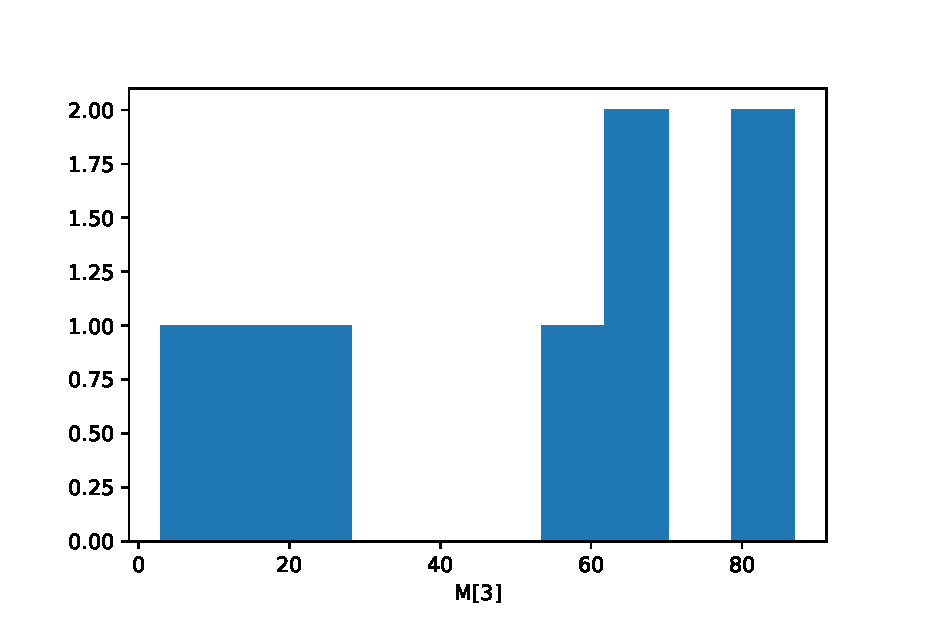
\includegraphics[scale=0.7]{hist1.eps}
\caption{Histogram of the 4th row of \textbf{M}.}
\label{F1}
\end{figure}
%%%%%%%%%%%%%%%%%%%%%%%%%%%%%%%%%%%%%%%%%%%%%%%%%%%%%
%
\begin{colorboxed}
\begin{lstlisting}[language={[ANSI]C},numbers=left,numberstyle=\tiny, frame=single, title=HW0\_4.1.py, breaklines=true,
   rulesepcolor=\color{red!20!green!20!blue!20},
   keywordstyle=\color{blue!70!black},
   commentstyle=\color{blue!90!},
   basicstyle=\ttfamily]
import numpy as np
import scipy.io as sio
import matplotlib.pyplot as plt
#load data
m = sio.loadmat('hw0data.mat')['M']
#print the dimensions of M.
print(np.ndim(m))
#print the 4th row and 5th column entry of M
print(m[3], m[:, 4])
#print the mean value of the 5th column of M
print(np.mean(m[:, 4]))
#compute the histogram of the 4th row of M and show the figure
plt.hist(m[3])
plt.show()
#compute and print the top three eigenvalues of the matrix MTM
evals, evecs = np.linalg.eig(np.dot(m.transpose(), m))
print(sorted(evals, reverse = True)[:3])
\end{lstlisting}
\end{colorboxed}

%%%%%%%%%%%%%%%%%%%%%%%%%%%%%%%%%%%%%%
\section*{Problem 4.2}
%
%%%%%%%%%%%%%%%%%%% Fig. 2 %%%%%%%%%%%%%%%%%%%%%%%%%%%%%%
\begin{figure}[ht]
\centering
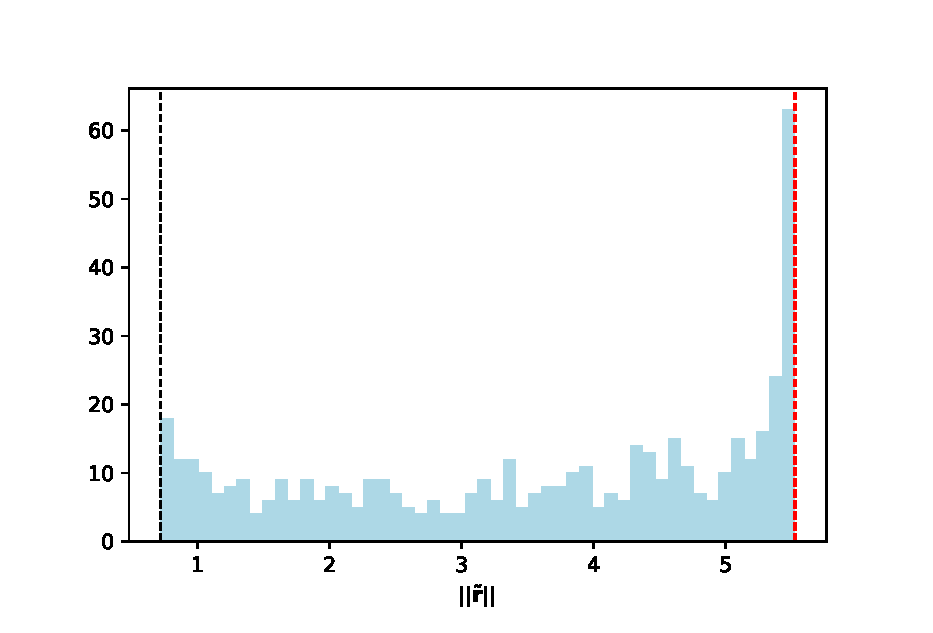
\includegraphics[]{hist2.eps}
\caption{Histogram of values of $||\tilde{\bf{r}}||$. Black dashed line is $\lambda_\mathrm{min}$ and red dashed line is $\lambda_\mathrm{max}$.}
\label{F2}
\end{figure}
%%%%%%%%%%%%%%%%%%%%%%%%%%%%%%%%%%%%%%%%%%%%%%%%%%%%%
%
\noindent (vii) From Fig.~\eqref{F2}, we could see that $||\tilde{\bf{r}}||$ lie between $\lambda_\mathrm{min}$ and $\lambda_\mathrm{max}$, which means $\lambda_\mathrm{min}$ is the lower bound of $||\tilde{\bf{r}}||$ while $\lambda_\mathrm{max}$ is the upper bound. 

\newpage
%
%%%%%%%%%%%%%%%%%%% Fig. 3 %%%%%%%%%%%%%%%%%%%%%%%%%%%%%%
\begin{figure}[ht]
\centering
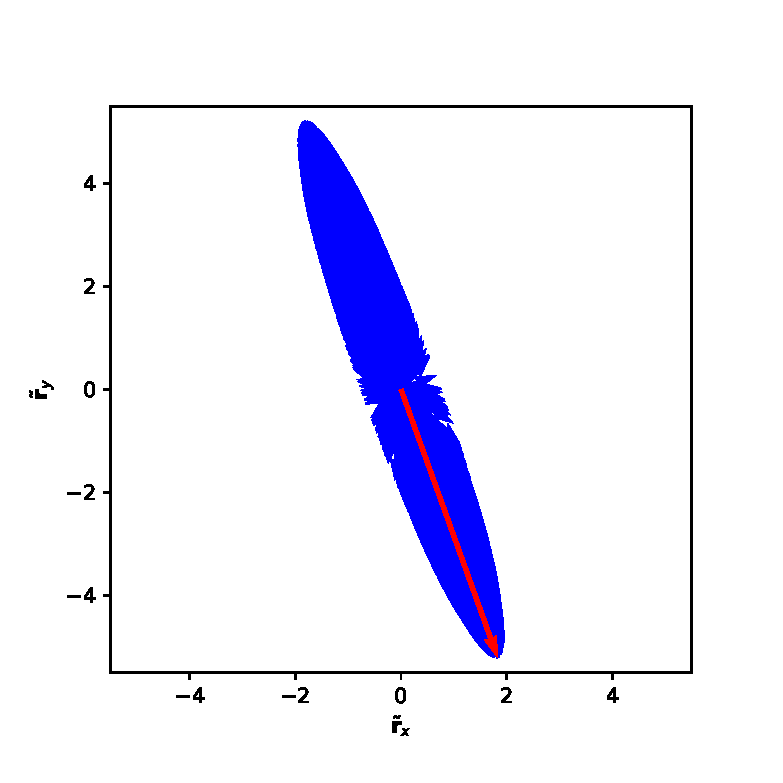
\includegraphics[]{fig3.eps}
\caption{2-D plot of all the distorted vectors $\tilde{\bf{r}}$ (in blue color) and $\bf{Lv}_{max}$ (in red color).}
\label{F3}
\end{figure}
%%%%%%%%%%%%%%%%%%%%%%%%%%%%%%%%%%%%%%%%%%%%%%%%%%%%%
%
\noindent (x) From Fig.~\eqref{F3}, we could see that $\bf{Lv}_{max}$ is the semi-major axis of the distribution of all the distorted vectors $\tilde{\bf{r}}$.
Since eigenvectors point in directions that are streched by the transformation from matrix $\bf{L}$, the eigenvector $\bf{v}_{max}$, which corresponds to the largest eigenvalue, points to the direction that is streched most severely. 
As a result, after the transformation of matrix $\bf{L}$, the set of vectors $\bf{r$ which originally have randomly distributed directions became a set of vectors $\tilde{\bf{r}}$ which have distorted distribution of directions. Most of them tend to point to the direction (or the reverse direction) of $\bf{v}_{max}$.

\begin{colorboxed}
\begin{lstlisting}[language={[ANSI]C},numbers=left,numberstyle=\tiny, frame=single, title=HW0\_4.2.py, breaklines=true,
   rulesepcolor=\color{red!20!green!20!blue!20},
   keywordstyle=\color{blue!70!black},
   commentstyle=\color{blue!90!},
   basicstyle=\ttfamily]
import numpy as np
import random
import matplotlib.pyplot as plt
nV = 500
#create a 2*2 matrix L
L = np.matrix([[5/4, -3/2], [-3/2, 5]])
#create a 2*500 array R to represent 500 random, unit length, 2-d vectors, in which R[:, i] is the i-th vector
R = np.zeros((2, nV))
for i in range(nV):
    tmp = np.array([random.gauss(0,1), random.gauss(0,1)])
    tmp = tmp/(sum(tmp * tmp) ** 0.5)
    R[:, i] = tmp
#compute R2 = LR, R2[:, i] is the distorted R[:, i]
R2 = np.dot(L,R)
#compute the eigenvalues of L and denote the minimum eigenvalue with lmax and lmin.
evals, evecs = np.linalg.eig(L)
[lMax, lMin] = sorted(evals, reverse = True)
#lr[i] is the length of the i-th vector in R2
lr = np.zeros((nV))
for i in range(nV):
    lr[i] = (np.dot(R2[:, i].transpose(), R2[:, i]))[0, 0] ** 0.5
#create a histogram of values of lr (use 50 bins) and compare it to lMax and lMin.
plt.hist(lr, bins = 50)
plt.axvline(lMax, color='r', linestyle='dashed', linewidth=1)
plt.axvline(lMin, color='k', linestyle='dashed', linewidth=1)
plt.show()
#compute the eigenvectors of L and Let vmax denote the eigenvector corresponding to the maximum eigenvalue lmax.
for i in range(2):
    if evals[i] == lMax: 
        vMax = evecs[:, i]
        break
#make a two-dimensional plot of R2 (in blue color) and the eigenvector vmax (in red color).
Lv = np.asarray(np.dot(L, vMax))
fig = plt.figure(figsize = (5, 5))
plt.quiver([0], [0], np.asarray(R2[0, :]), np.asarray(R2[1, :]), color = 'b', angles='xy', scale_units='xy', scale=1)
plt.quiver([0], [0], Lv[0], Lv[1], color = 'r', angles='xy', scale_units='xy', scale=1)
plt.xlim(-5.5, 5.5)
plt.ylim(-5.5, 5.5)
plt.show()
\end{lstlisting}
\end{colorboxed}



 

\end{document} 
